\section{Feature-Auswahl, Hyperparametersuche und Modellauswahl} \label{sec:Ergeb FeatSel,Hyp,ModSel}
Um eine optimale Feature-Menge zu finden, wird aus einer Reihe von Versuchen mit Wrapper-Methoden eine Feature-Rangfolge abgeleitet. Um die Feature-Menge unabhängig vom Modell zu beurteilen, wird die Accuracy von mehreren Modellen validiert und anschließend gemittelt. In diesem Kapitel werden die Feature-Rangfolgen der Filter-Methoden betrachtet. Damit wird die konstruierte Rangfolge aus dem Wrapper-Score verglichen. Es wird untersucht, ob sich das Entfernen von Features, die auf dem gleichen Basis-Feature aufbauen, positive auswirkt. Ebenfalls wird untersucht, ob alle Feature-Kategorien benötigt werden. Abschließen tut das Kapitel mit dem Vergleich der betrachteten Modelle und dem finalen Test des ausgewählten Modells.\par

Ziel der Untersuchung ist es, für das Modul das bestmögliche Modell zu schaffen. Zu suchen ist eine Feature-Menge und ein Modell, welche besser performen, als andere Feature-Mengen oder Modelle. Zu berücksichtigen ist die Verarbeitungszeit. Für das Modul ist eine kleine Feature-Menge vorteilhafter für die Echtzeitfunktionalität. \par


\subsection{Vergleich der Filter-Methoden mit der entworfenen Rangfolge}
Die Plots in der Abbildung \ref{fig:plotMethVergl} zeigen den Verlauf der Accuracy in Bezug zur Feature-Menge gemäß der jeweiligen Rangfolge. Dargestellt sind die Varianzanalyse, die gegenseitige Information und der Wrapper-Score. Zur besseren Vergleichbarkeit sind die Sättigungskurve eingezeichnet. Die Tabelle \ref{tab:FiltVsWrap} zeigt einen tabellarischen Vergleich.

\begin{figure}[htbp]
     \centering
     \begin{subfigure}[b]{0.9\textwidth}
         \centering
         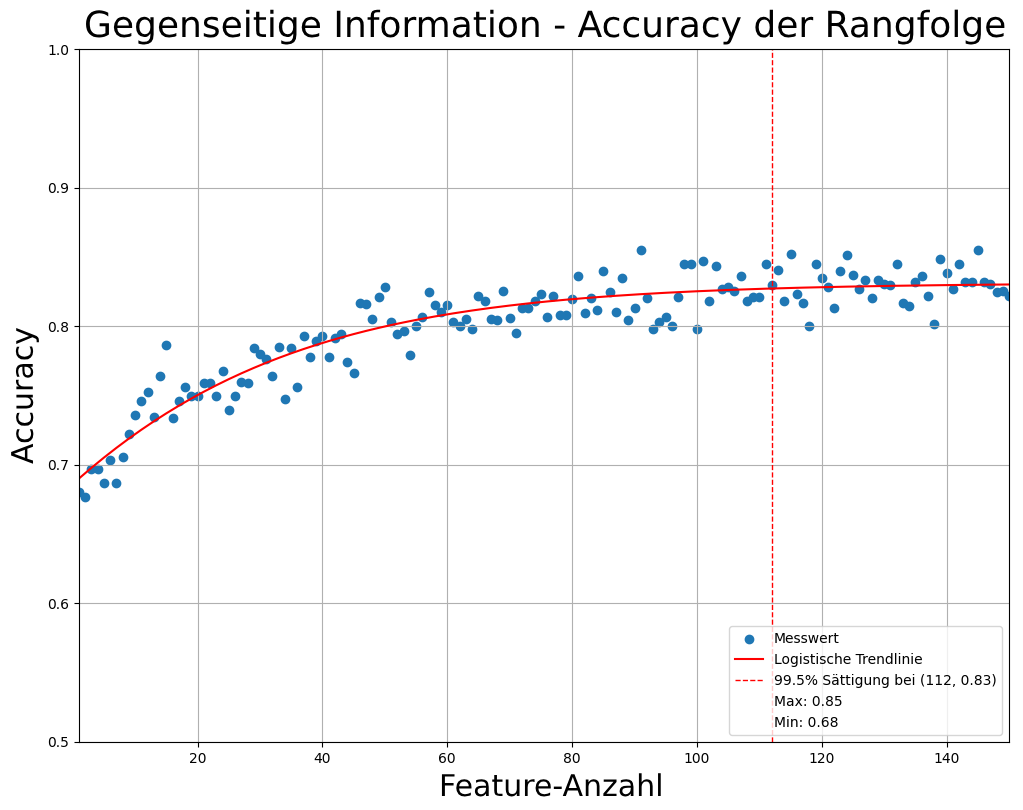
\includegraphics[width=\textwidth, height=11cm]{img/Plots/Feature Auswahl/Filter-Methoden Mutual Info.png}
         \caption{Varianzanalyse}
     \end{subfigure}
     \hfill
     \begin{subfigure}[b]{0.9\textwidth}
         \centering
         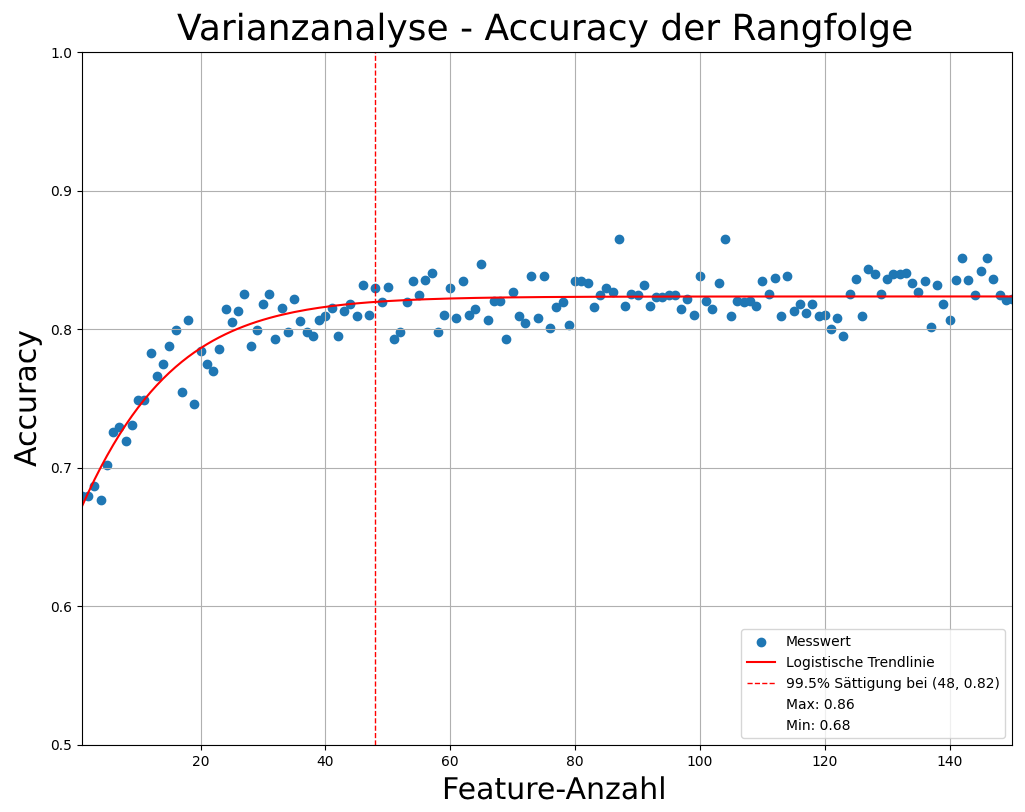
\includegraphics[width=\textwidth, height=11cm]{img/Plots/Feature Auswahl/Filter-Methoden ANOVA.png}
         \caption{Gegenseitige Information}
     \end{subfigure}
     \caption{Verlauf der Accuracy der Filter-Methoden und der entworfenen Rangfolge.}
     \label{fig:plotMethVergl}
\end{figure}

\begin{table}[htbp]
\centering
\caption{Vergleich der Sättigungspunkte der Rangfolgen.}
\label{tab:FiltVsWrap}
\begin{tabular}{
  >{\raggedright\arraybackslash}p{0.4\linewidth}
  S[table-format=2.0]
  S[table-format=3.0]
}
\toprule
{Methode} & {Accuracy [\%]} & {Featureanzahl} \\
\midrule
Varianzanalyse & 82 & 48 \\
gegenseitige Information & 83 & 112 \\
Wrapper-Score & 85 & 36 \\
\bottomrule
\end{tabular}
\end{table}

Es ist zu sehen, dass die Rangfolge nach dem Wrapper-Score im besten Verlauf der Accuracy resultiert. Die Sättigung wird mit der kleinsten Feature-Menge erreicht und die Accuracy ist im Vergleich am höchsten. Das legitimiert das Vorgehen. \par

Wie in \autoref{sec:Meth KonstrFeatures} dargestellt, liegt die Feature-Anzahl bei 3114. Die Plots zeigen, dass nur ein Bruchteil dieser Menge notwendig ist, um die Sättigung zu erreichen. Das spricht für viel Redundanz in den Features.


\subsection{Auswirkungen der Entfernung von Features gleicher Basis} \label{sec:Ergeb FeatKategories}

\begin{figure}[hp]
     \centering
     \begin{subfigure}[b]{0.9\textwidth}
         \centering
         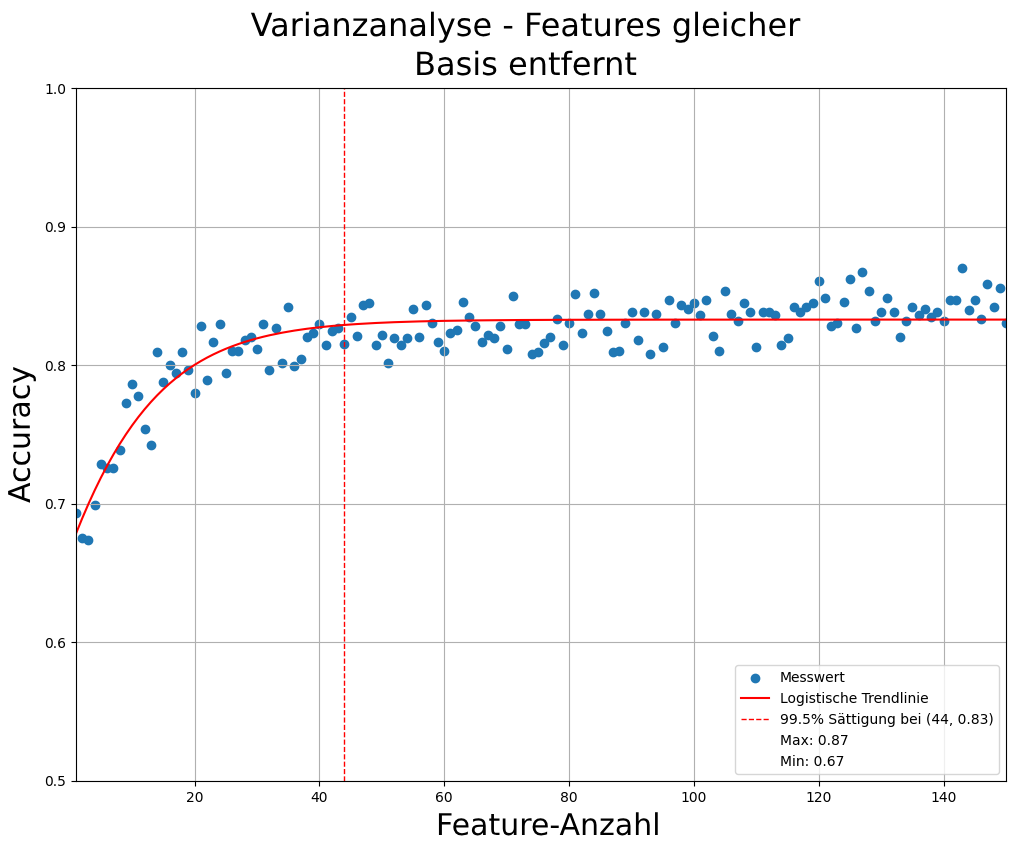
\includegraphics[width=\textwidth, height=11cm]{img/Plots/Feature Auswahl/Filter-Methoden ANOVA mit Entfernen.png}
         \caption{Varianzanalyse}
     \end{subfigure}
     \hfill
     \begin{subfigure}[b]{0.9\textwidth}
         \centering
         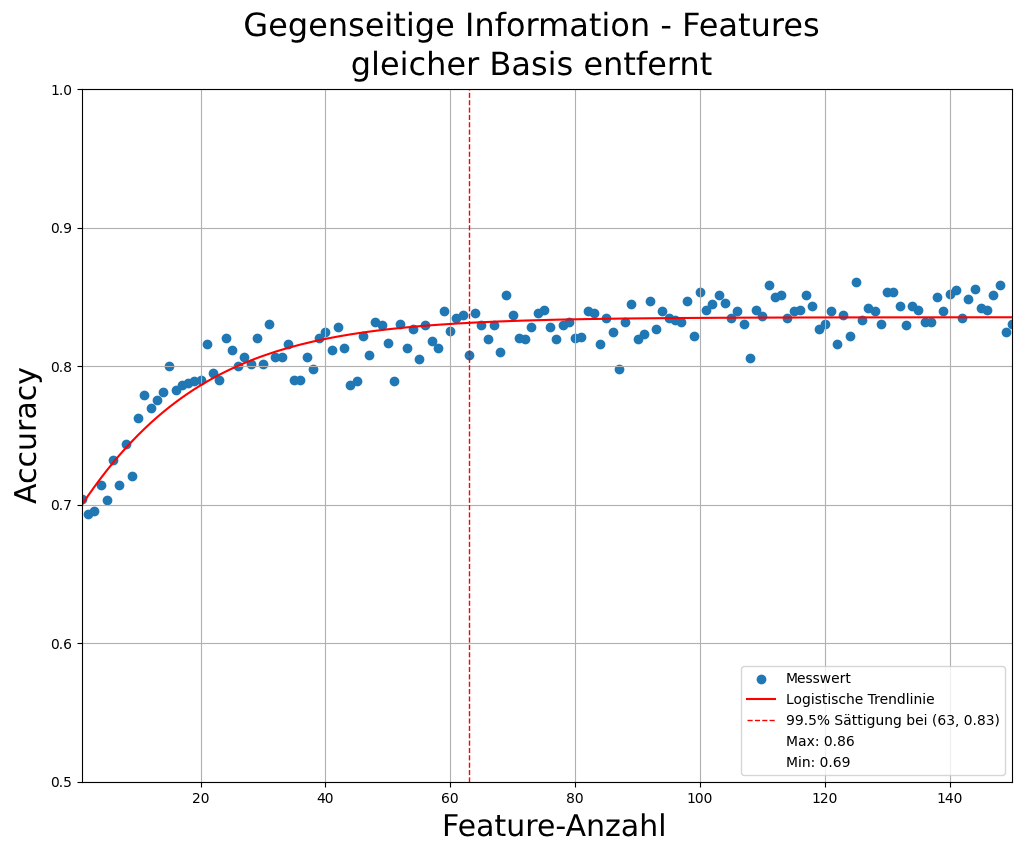
\includegraphics[width=\textwidth, height=11cm]{img/Plots/Feature Auswahl/Filter-Methoden Mutual Info mit Entfernen.png}
         \caption{Gegenseitige Infomation}
     \end{subfigure}
     \caption{Verlauf der Accuracy nach dem Entfernen von Features mit gleicher Basis.}
     \label{fig:plotRIPsame Bais}
\end{figure}

\begin{figure}[hp]
     \centering
     \begin{subfigure}[b]{0.9\textwidth}
         \centering
         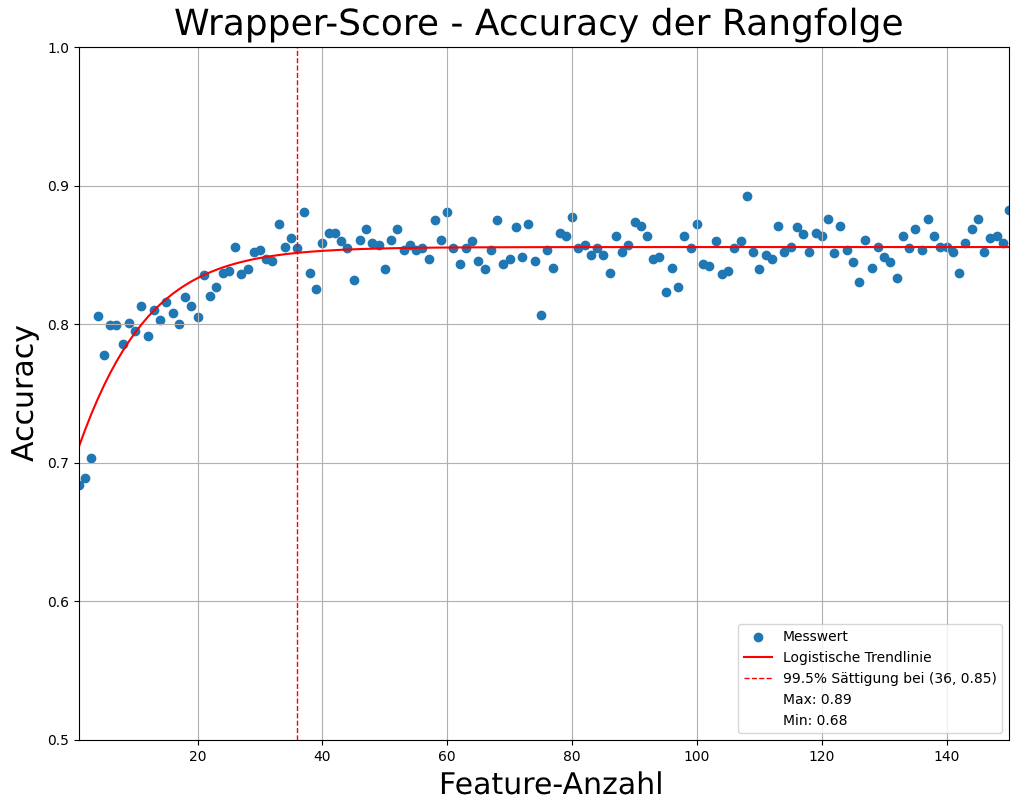
\includegraphics[width=\textwidth, height=11cm]{img/Plots/Feature Auswahl/Wrapper-Score.png}
         \caption{Wrapper-Score voher}
     \end{subfigure}
     \hfill
     \begin{subfigure}[b]{0.9\textwidth}
         \centering
         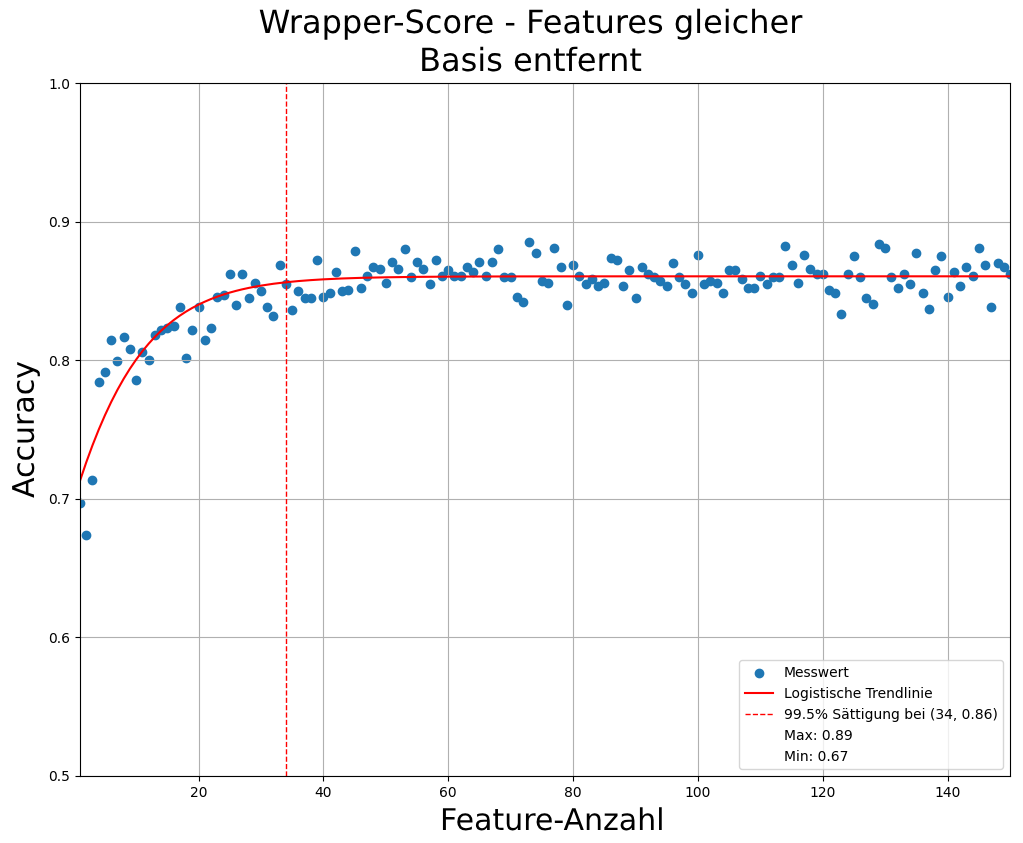
\includegraphics[width=\textwidth, height=11cm]{img/Plots/Feature Auswahl/Wrapper-Score mit Entfernen.png}
         \caption{Wrapper-Score nachher}
     \end{subfigure}
     \caption{Verlauf der Accuracy nach dem Entfernen von Features mit gleicher Basis.}
     \label{fig:plotRIPsame Bais Wrap}
\end{figure}

Die Rangfolgen werden bearbeitet. Von den Features, die auf dem gleichen Basis-Feature aufbauen, befindet sich schließlich nur noch das Höchstrangige in der Rangfolge. Dadurch soll Redundanz reduziert werden. In der Abbildung \ref{fig:plotRIPsame Bais} sind die entsprechenden Plots zu den Rangfolgen der Filter-Methoden zu sehen und in der Abbildung \ref{fig:plotRIPsame Bais Wrap} sind die des Wrapper-Scores zu sehen. In der Tabelle \ref{tab:entfSameBasis} befindet sich ein tabellarischer Vergleich.

\begin{table}[htbp]
\centering
\caption{Vergleich der Sättigungspunkte nach entfernen von Features gleicher Basis.}
\label{tab:entfSameBasis}
\begin{tabular}{
  >{\raggedright\arraybackslash}p{0.4\linewidth}
  S[table-format=2.0]
  S[table-format=3.0]
}
\toprule
{Methode} & {Accuracy [\%]} & {Featureanzahl} \\
\midrule
Varianzanalyse & 83 & 44 \\
gegenseitige Information & 83 & 63 \\
Wrapper-Score & 86 & 34 \\
\bottomrule
\end{tabular}
\end{table}

Es ist zu sehen, dass sich das Entfernen von Features, mit gleicher Basis, auf alle Feature-Rangfolgen positiv ausgewirkt. Es wird eine bessere Accuracy mit weniger Features erreicht. Somit lässt sich sagen, dass tatsächlich Redundanzen entfernt werden, wodurch eine Feature-Menge entsteht, welche dem Modell mehr Information bietet als zuvor.

\clearpage
\subsection{Performancevergleich der Feature-Kategorien}
Aus der Rangfolge des Wrapper-Scores werden nur bestimmte Feature-Kategorien und Kombinationen von Kategorien getestet. Die Verläufe der Accuracy sind in der Abbildung \ref{fig:plotCompKateg} zu sehen. Eine tabellarische Darstellung befindet sich in der Tabelle \ref{tab:comKate}.

\begin{figure}[htb]
     \centering
     \begin{subfigure}[b]{\textwidth}
         \begin{subfigure}[b]{0.49\textwidth}
             \centering
             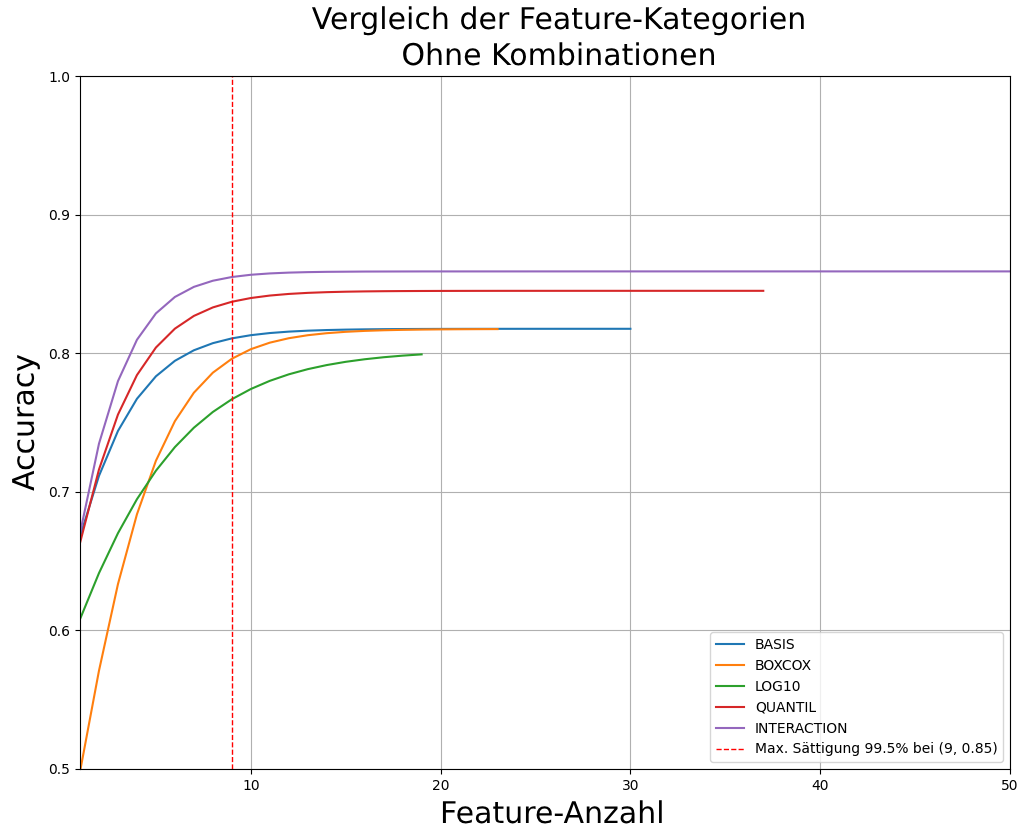
\includegraphics[width=\textwidth]{img/Plots/Feature Auswahl/Trendlinien Feature-Kategorien 0Up- Accuracy Plot.png}
             \caption{Keine Kombinationen}
         \end{subfigure}
         \hfill
         \begin{subfigure}[b]{0.49\textwidth}
             \centering
             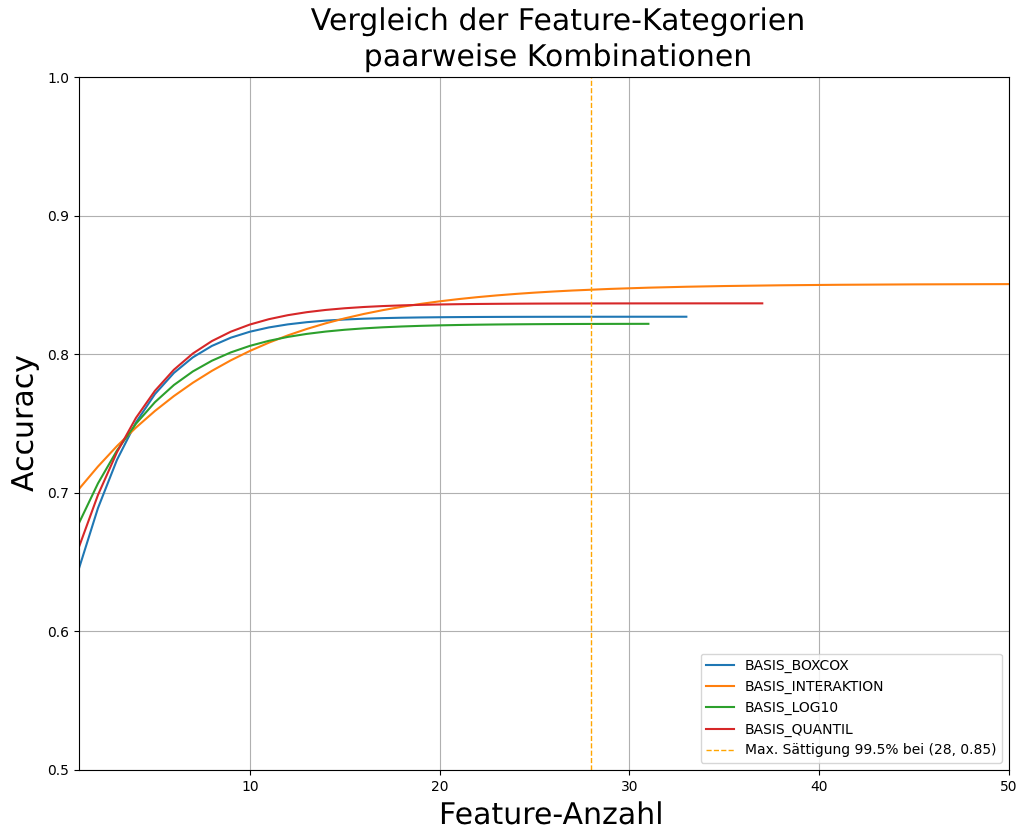
\includegraphics[width=\textwidth]{img/Plots/Feature Auswahl/Trendlinien Feature-Kategorien 1Up - Accuracy Plot.png}
             \caption{Einfache Kombinationen}
         \end{subfigure}
     \end{subfigure}
     \hfill
     \begin{subfigure}[b]{\textwidth}
         \begin{subfigure}[b]{0.49\textwidth}
             \centering
             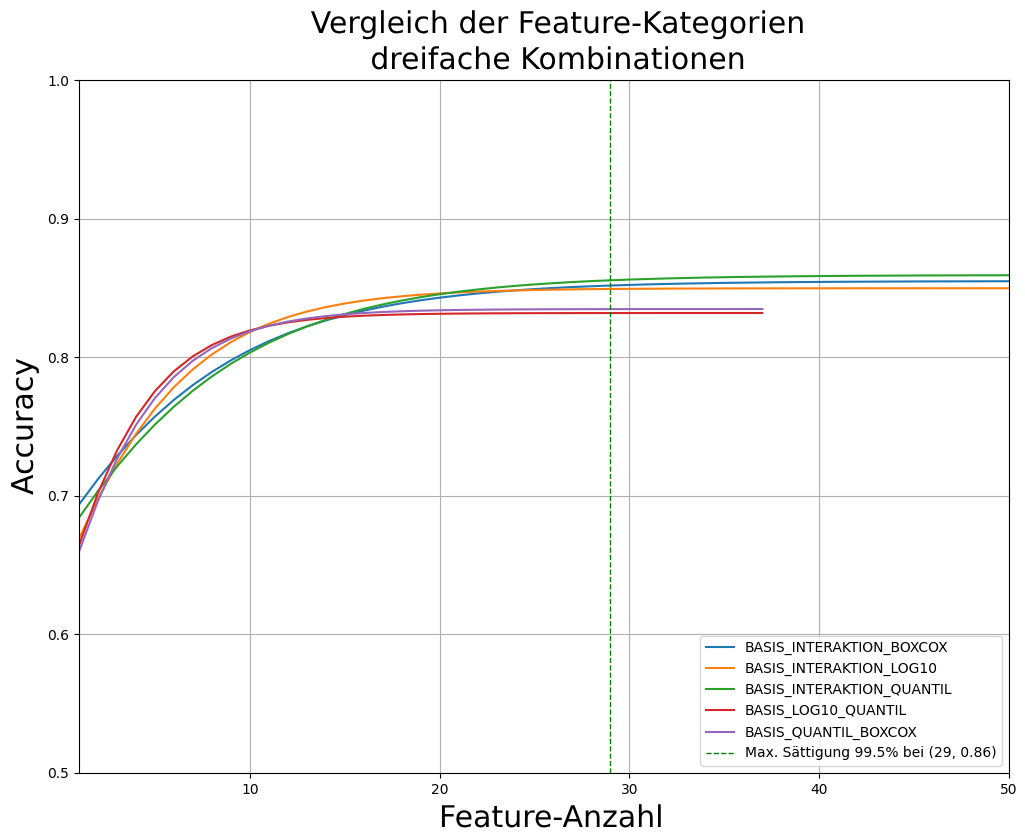
\includegraphics[width=\textwidth]{img/Plots/Feature Auswahl/Trendlinien Feature-Kategorien 2Up - Accuracy Plot.png}
             \caption{Zweifache Kombinationen}
         \end{subfigure}
         \hfill
         \begin{subfigure}[b]{0.49\textwidth}
             \centering
             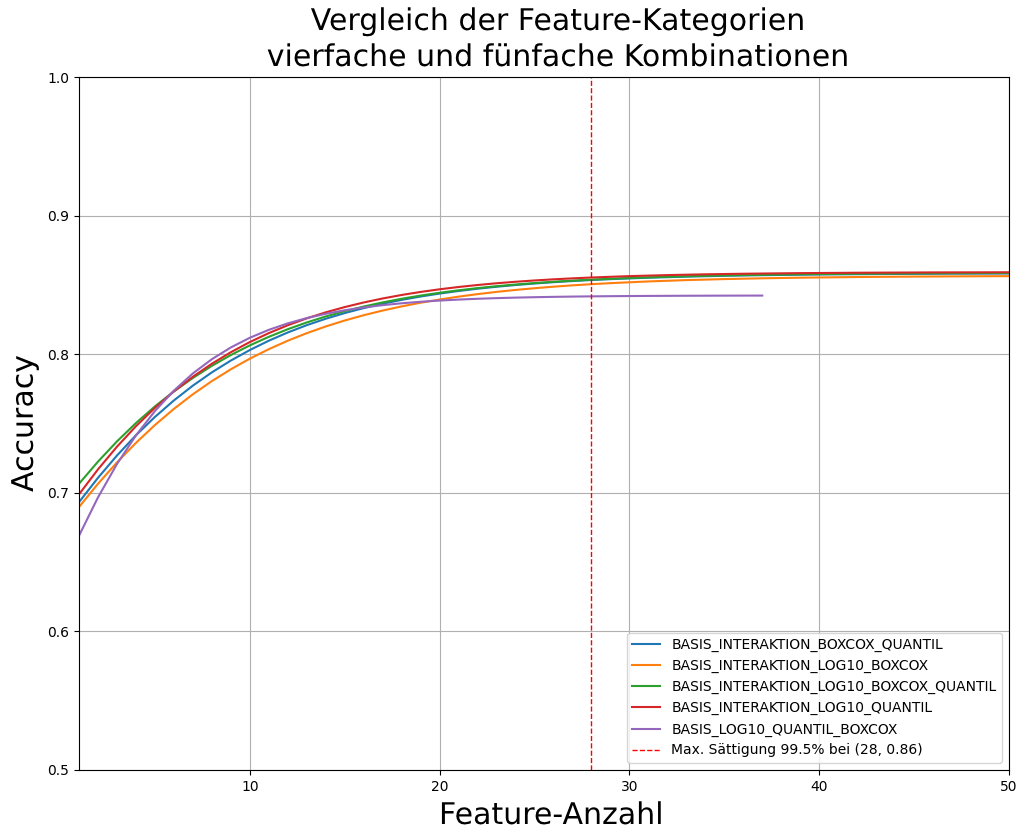
\includegraphics[width=\textwidth]{img/Plots/Feature Auswahl/Trendlinien Feature-Kategorien 3Up - Accuracy Plot.png}
             \caption{Vier- und fünffache Kombinationen}
         \end{subfigure}
     \end{subfigure}
     \caption{Verlauf der Accuracy von unterschiedlichen Kombinationen der Feature-Kategorien.}
     \label{fig:plotCompKateg}
\end{figure}

\begin{table}[htbp]
\centering
\caption{Vergleich der Sättigungspunkte unterschiedlicher Kategorie-Kombinationen}
\label{tab:comKate}
\begin{tabular}{
  >{\raggedright\arraybackslash}p{0.5\linewidth}
  S[table-format=2.0]
  S[table-format=2.0]
}
\toprule
{Kombination} & {Accuracy [\%]} & {Featureanzahl} \\
\midrule
Basis & 81 & 11 \\
Interaktion & 85 & 9 \\
Quantil & 84 & 11 \\
Log & 82 & 16 \\
BoxCox & 81 & 14 \\
\midrule
Basis-Interaktion & 85 & 28 \\
Basis-Quantil & 83 & 15 \\
Basis-Log & 82 & 16 \\
Basis-BoxCox & 82 & 13 \\
\midrule
Basis-Interaktion-Quantil & 86 & 29 \\
Basis-Interaktion-Log & 85 & 20 \\
Basis-Interaktion-BoxCox & 85 & 28 \\
Basis-Quantil-Log & 83 & 14 \\
Basis-Quantil-BoxCox & 83 & 15 \\
Basis-Log-BoxCox & 82 & 14 \\
\midrule
Basis-Interaktion-Quantil-Log & 86 & 28 \\
Basis-Interaktion-Quantil-BoxCox & 85 & 30 \\
Basis-Interaktion-Log-BoxCox & 85 & 31 \\
Basis-Quantil-Log-BoxCox & 84 & 20 \\
\midrule
Basis-Interaktion-Quantil-Log-BoxCox & 85 & 30 \\
\bottomrule
\end{tabular}
\end{table}

Es ist zu sehen, dass die höchste Accuracy mit der Kombination aus den Basis-Features, den Interaktionsfeatures und den Quantil-Features erreicht wird, oder mit der gleichen Kombination, mit den logarithmischen Features zusätzlich. Im zweiten Fall wird die Sättigung mit einem Feature weniger erreicht. Um die Berechnung der logarithmischen Features einzusparen, wird sich für die erste Kombination entschieden.\par

Die Box-Cox-Features und die logarithmischen Features werden nicht verwendet für das Modul.


\subsection{Untersuchungen zur Modellauswahl} \label{sec:ErgebModSelEval}
Die Abbildung \ref{fig:plotCompModel} zeigt die Plots der Accuracy zu den unterschiedlichen Modellen. In der Tabelle \ref{tab:compModel} ist der Vergleich der Sättigungspunkte zu sehen.

\begin{figure}[p]
     \centering
     \begin{subfigure}[b]{0.9\textwidth}
         \begin{subfigure}[b]{0.49\textwidth}
             \centering
             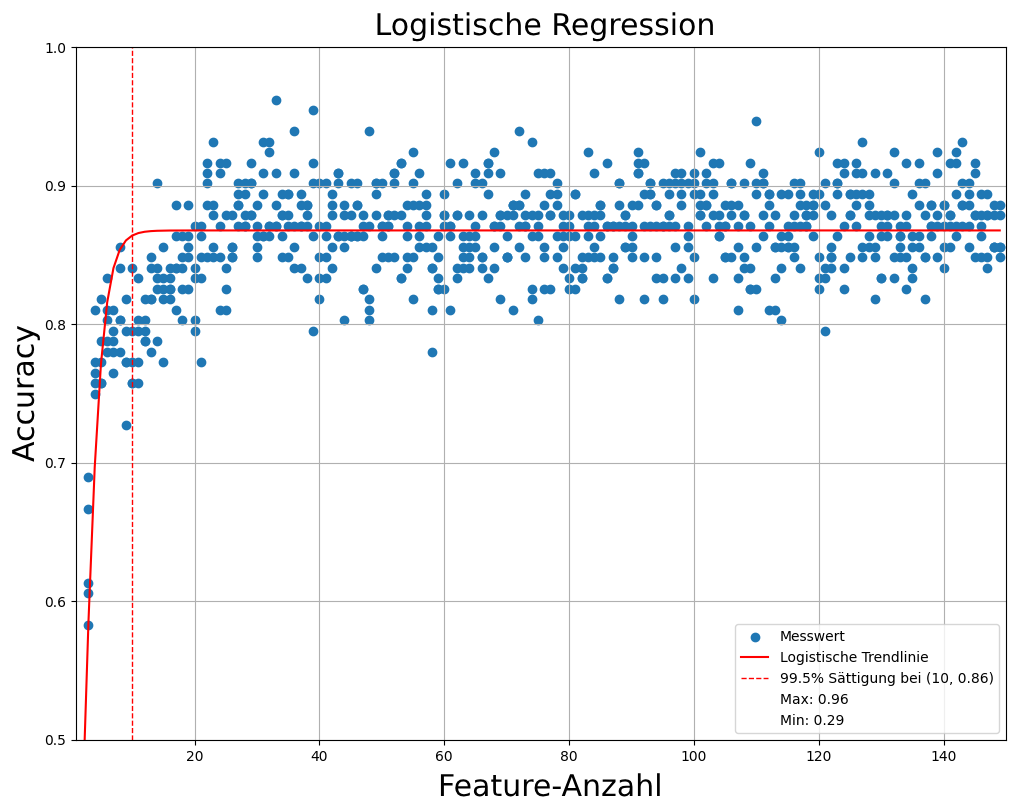
\includegraphics[width=\textwidth, height=5cm]{img/Plots/Modell Auswahl/Logistic Regression - Accuracy Plot.png}
             \caption{Logistische Regression}
         \end{subfigure}
         \hfill
         \begin{subfigure}[b]{0.49\textwidth}
             \centering
             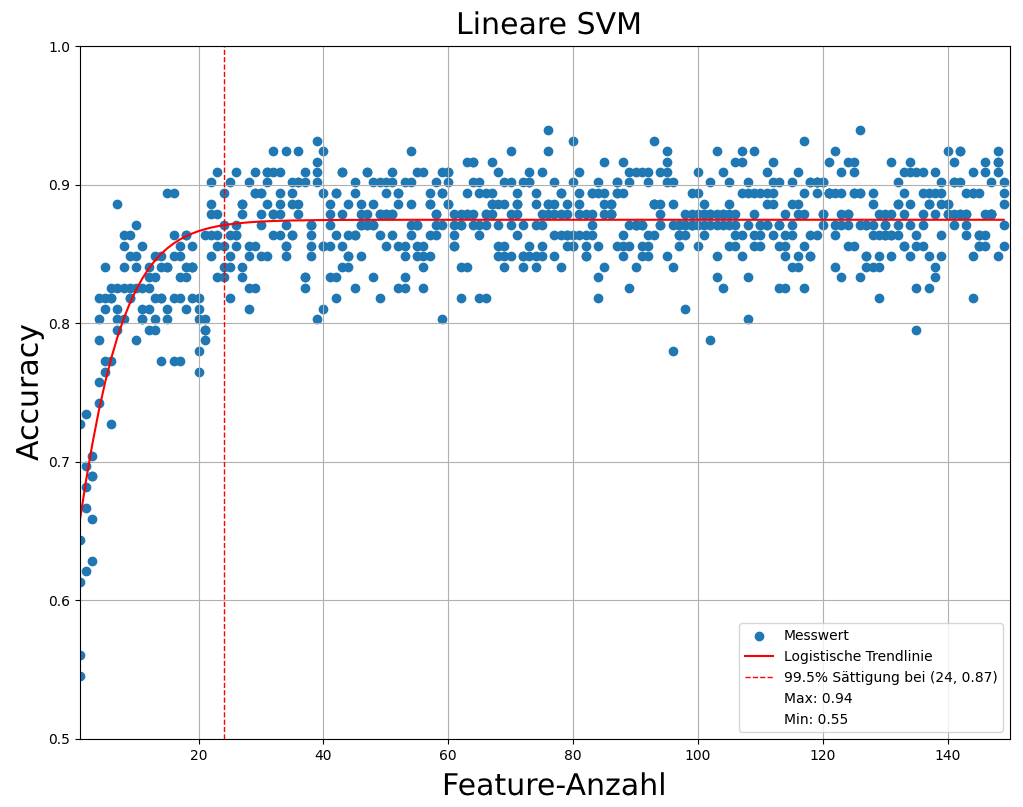
\includegraphics[width=\textwidth, height=5cm]{img/Plots/Modell Auswahl/Linea SVM - Accuracy Plot.png}
             \caption{Lineare SVM}
         \end{subfigure}
     \end{subfigure}
     \hfill
     \begin{subfigure}[b]{0.9\textwidth}
         \begin{subfigure}[b]{0.49\textwidth}
             \centering
             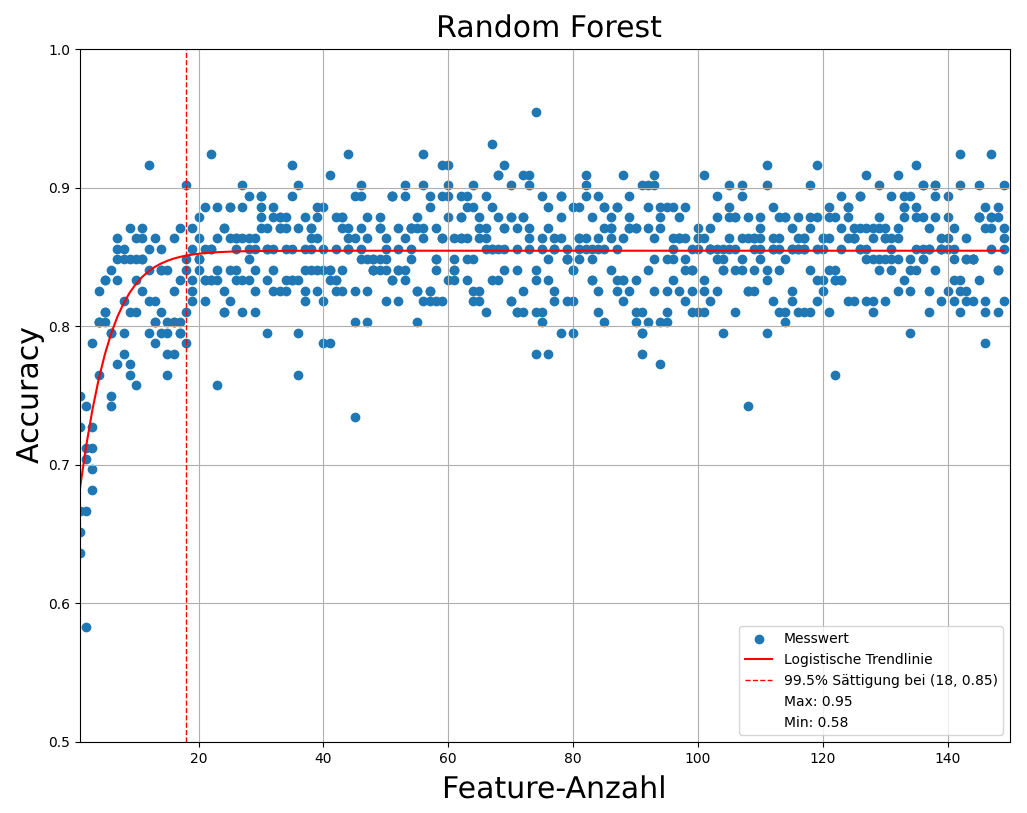
\includegraphics[width=\textwidth, height=5cm]{img/Plots/Modell Auswahl/Random Forest - Accuracy Plot.png}
             \caption{Random Forest}
         \end{subfigure}
         \hfill
         \begin{subfigure}[b]{0.49\textwidth}
             \centering
             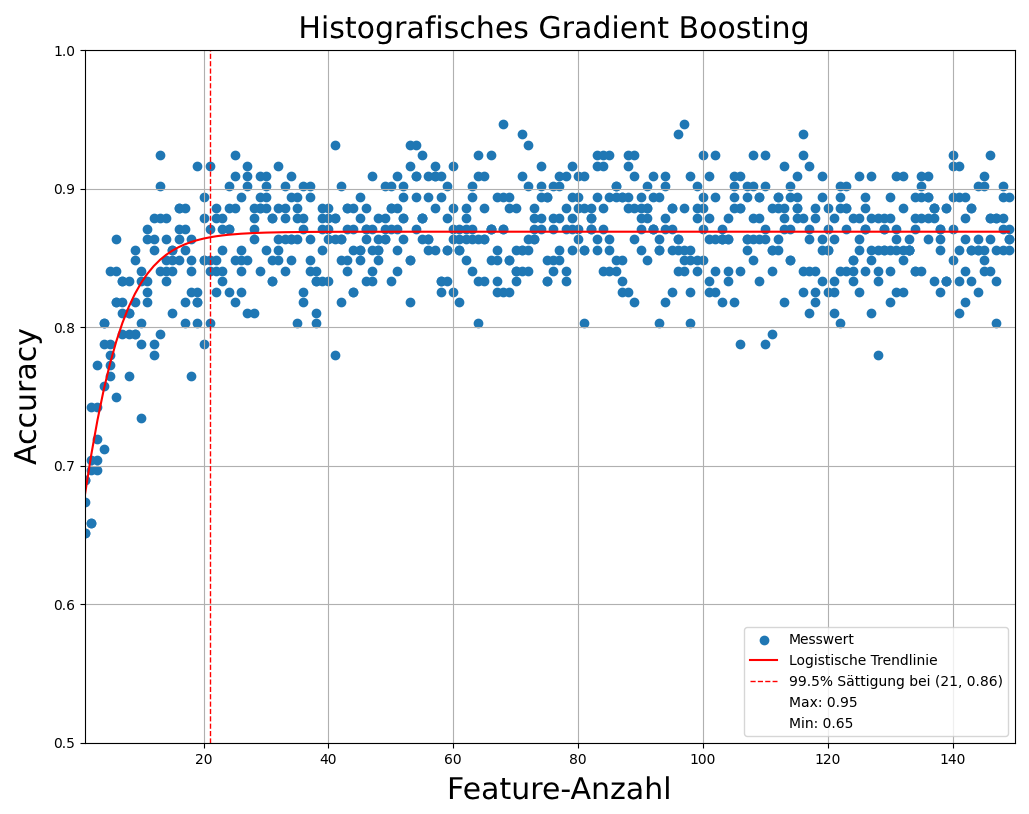
\includegraphics[width=\textwidth, height=5cm]{img/Plots/Modell Auswahl/Hist Gradien Boosting - Accuracy Plot.png}
             \caption{Histografisches Gradient Boosting}
         \end{subfigure}
     \end{subfigure}
     \begin{subfigure}[b]{0.9\textwidth}
         \centering
         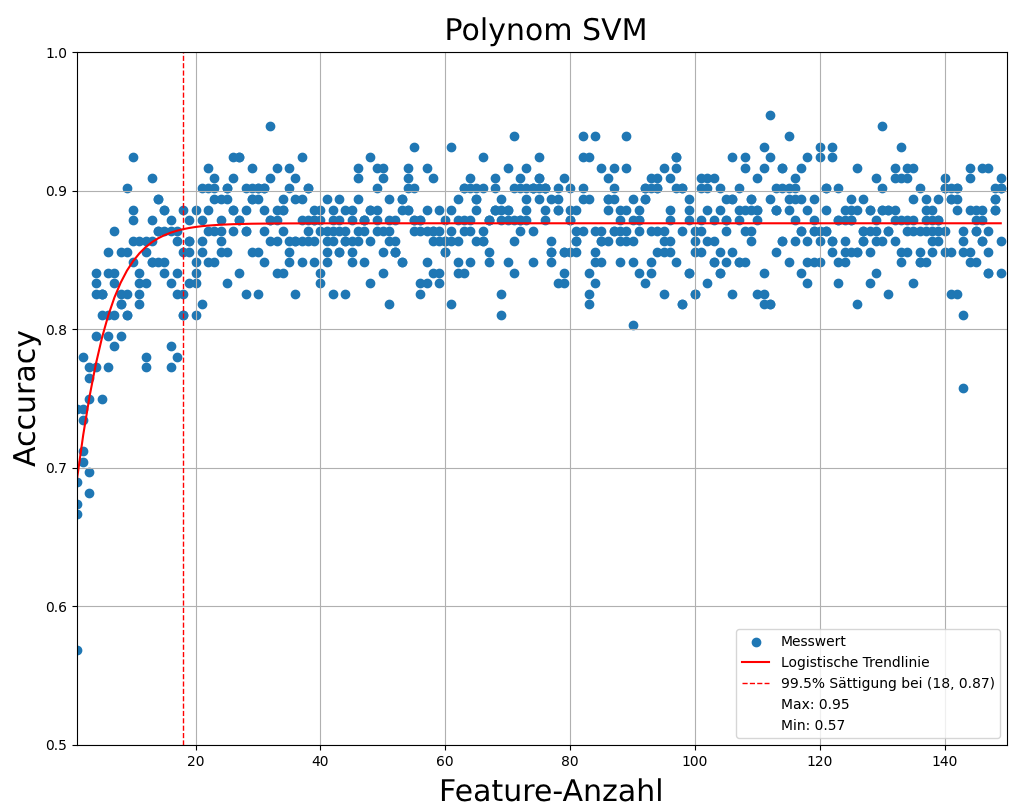
\includegraphics[width=\textwidth, height=10cm]{img/Plots/Modell Auswahl/poly SVM - Accuracy Plot.png}
         \caption{Polynomiale SVM}
     \end{subfigure}
     \caption{Verlauf der Accuracy der unterschiedlichen Modelle.}
     \label{fig:plotCompModel}
\end{figure}

\begin{table}[htbp]
\centering
\caption{Vergleich der verschiedenen Modelle}
\label{tab:compModel}
\begin{tabular}{
  >{\raggedright\arraybackslash}p{0.5\linewidth}
  S[table-format=2.0]
  S[table-format=2.0]
}
\toprule
{Modelle} & {Accuracy [\%]} & {Featureanzahl} \\
\midrule
logistische Regression & 86 & 10 \\
lineare SVM & 87 & 24 \\
polynomiale SVM & 87 & 18 \\
Random Forest & 85 & 18 \\
Histografisches Gradient Boosting & 86 & 21 \\
\bottomrule
\end{tabular}
\end{table}

Es ist zu sehen, dass Unterschiede in der Performance zwischen den Modellen, nach der Hyperparametersuche kaum vorhanden sind. Die niedrigste Feature-Anzahl benötigt die logistische Regression. Bei Betrachtung der Abbildung \ref{fig:plotCompModel} wirkt es jedoch so, dass die Sättigungskurve hier den Verlauf nicht richtig approximiert. Der tatsächliche Sättigungspunkt wird ebenfalls bei ca. 20 Features erreicht. Am besten schneiden die SVMs ab. Die polynomiale SVM erreicht die Sättigung mit einer etwas kleineren Feature-Anzahl als die lineare SVM. Aus diesem Grund fällt die Entscheidung auf die polynomiale SVM.

Die Abbildung \ref{fig:plotTrainTestFinal} zeigt den Vergleich der Accuracy des Trainings, der Validierung und des Testens. Es ist zu sehen, dass die Wertungen nah aneinander verlaufen. Dadurch ist auszuschließen, dass das Modell overfittet. Dass der Trainingswert etwas besser ist, als der Validierungswert und der Testwert ist üblich und zu erwarten. 

\begin{figure}[htb]
    \centering
    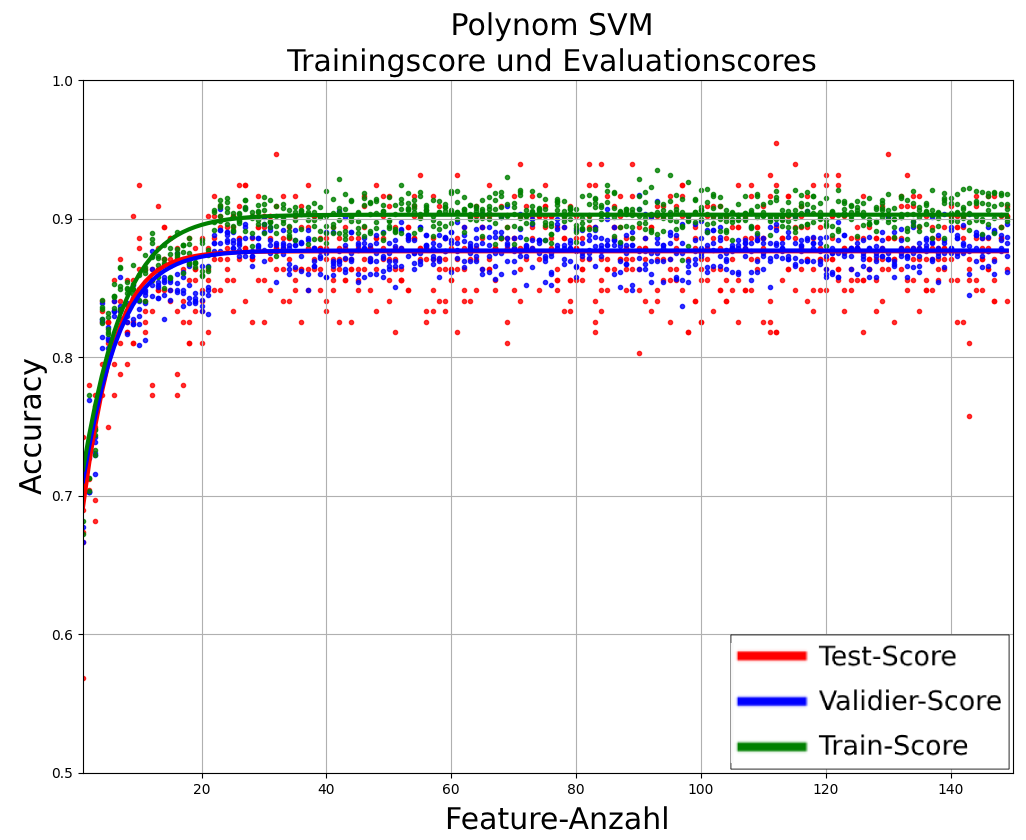
\includegraphics[width=0.9\textwidth]{img/Plots/Modell Auswahl/poly SVM - Comparation Plot.png}
    \caption{Verlauf der Accuracy des Trainings, der Validierung und des Testens des finalen Modells.}
    \label{fig:plotTrainTestFinal}
\end{figure}

Die Tabelle \ref{tab:KonfMatr} zeigt die Konfusionsmatrix des finalen Tests.

\begin{table}[htbp]
    \centering
    \caption{Konfusionsmatrix des Testens des finalen Modells.}
    \label{tab:KonfMatr}
    \begin{tabular}{l|rrr|r}
        \toprule
        \multirow{1}{*}{\textbf{Echtes Verhalten}} & \multicolumn{3}{c|}{\textbf{Geschätztes Verhalten}} & {\textbf{Gesamt}}\\
        %\cmidrule(lr){2-4}
         & Kampf & Kontrollgang & Normalverhalten & \\
        \midrule
        Kampf                & 82,0\, \% &  2,6\, \% & 16,0\, \% & 100 \%\\
        Kontrollgang         &  2,3\, \% & 98,0\, \% &  0,0\, \% & 100 \%\\
        Normalverhalten      & 12,0\, \% &  0,0\, \% & 88,0\, \% & 100 \%\\
        \bottomrule
    \end{tabular}
\end{table}

\clearpage
\subsection{Fazit der Untersuchungen zur Feature-Auswahl und der Modellauswahl}
Die Ermittlung der Feature-Rangfolge über den Wrapper-Score übertrifft die der Filter-Methoden. Dadurch ist bestätigt, dass multivariate Einflüsse Modell unabhängig berücksichtigt werden. Das Entfernen von Features, die sich die Basis teilen, reduziert Redundanz und verbesser die Feature-Rangfolge. Für eine gute Performance ist es ausreichend nur die Basis-Features, die Quantil-Features und die Interaktionsfeatures zu ermitteln. Mit dieser Rangfolge und den eingestellten Hyperparametern sind nur kleine Unterschiede in der Performance der Modelle festzustellen. Mit der polynomialen SVM lässt sich laut den Daten die beste Accuracy mit der kleinsten Feature-Anzahl erreichen. Dieses Modell wird ausgewählt. Um stabiler in der Sättigung zu liegen wird die Feature-Anzahl auf 40 vergrößert.